\part[总述]{总述}
本指南含成绩计算、学分、绩点,缓考、补考、重修,三阶段考试等内容,旨在解答同学们对分数计算以及三阶段考试的相关疑惑。

本节内容参考自以下文件:山二医教字〔2025〕4号《山东第二医科大学普通全日制本科学生学士学位授予工作办法(修订)》、山二医教字〔2025〕5号《山东第二医科大学考试工作管理办法(修订)》、山二医教字〔2025〕6号《山东第二医科大学课程重修管理办法》、山二医教字〔2025〕7号《山东第二医科大学本科生学业预警管理办法(修订)》、山二医教字〔2025〕12号《山东第二医科大学临床医学类专业“三阶段”综合考试实施方案(修订)》、教务处《山东第二医科大学本科专业人才培养方案(2021版)》、教务处《山东第二医科大学2024年普通全日制本科学生转专业工作方案》等。因文章长度所限此处无法一一列举,不甚清晰之处敬请参阅各文件的对应章节。

\newpage
\part[分数计算]{分数计算}

\section[成绩]{成绩}
\label{score}
注:本节所用的“成绩”一词如无特殊说明均指代\textbf{“综合成绩}”。
\begin{enumerate}
    \item 各科成绩满分为100分,及格为60分
    \item 成绩由“平时成绩”与“期末成绩”组成,此两项满分均为100分,及格均为60分;最终加权得到综合成绩,详见下表
    \item 非限选课的“划线”(即,计算综合成绩时计入平时成绩所需的最低期末考试分数)由任课教师及相关教研室决定
    \item 成绩及格即可取得该科的学分与绩点,否则需要补考或重修
\end{enumerate}

\noindent\makebox[\textwidth][c]{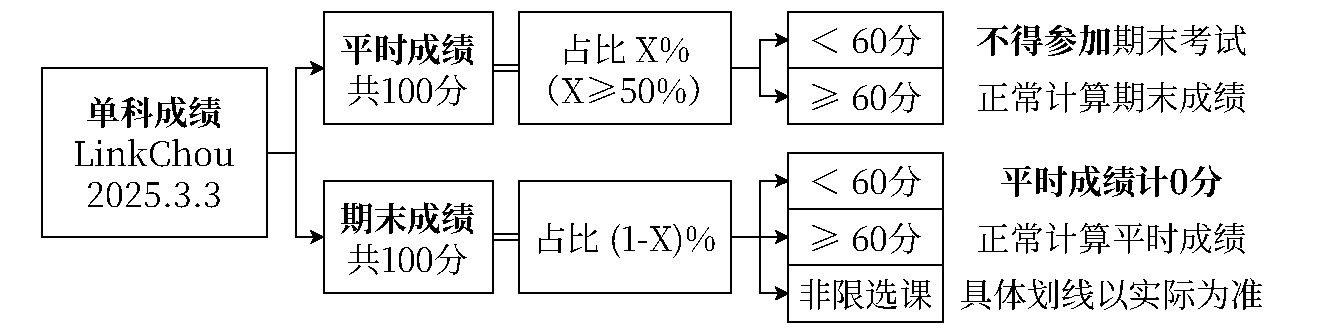
\includegraphics[width=\textwidth]{单科成绩计算.pdf}}

\subsection[绩点]{绩点}
\label{gpa} % grade point average
\begin{enumerate}
    \item \textbf{平均学分绩点(GPA) ≥ 2}是获得学位证的要求之一
    \item 绩点计算方式如下:
          \begin{enumerate}
              \item \textbf{课程绩点}(综合成绩不及格,绩点记为0分):
                    \begin{equation}
                        \frac{课程综合成绩}{10} - 5
                    \end{equation}
              \item \textbf{平均学分绩点(GPA)}(平均绩点):
                    \begin{equation}
                        \frac{\sum (课程绩点 \times 课程学分)}{\sum 课程学分}
                    \end{equation}
          \end{enumerate}
    \item 补考合格的科目按60分计,换算后为1绩点,其他特殊情景参考\uref{retake}小节
\end{enumerate}

\subsection[学分]{学分}
\begin{enumerate}
    \item 需修满对应的学分方可授予学位证
    \item 学分还用于学费计算(每分100元,其余不再赘述)
    \item 特殊事项:“公共选修课联盟”的公共选修课程不算学分、不收学费
    \item 各类学分要求详表\footnotemark 如下图所示
\end{enumerate}
\footnotetext{因不同学制、学院、年级要求各不相同,本图仅以\textbf{2021级临床医学院临床医学系普通5年制本科}为例,其他内容请参阅对应的“培养方案”。}

\noindent\makebox[\textwidth][c]{%
    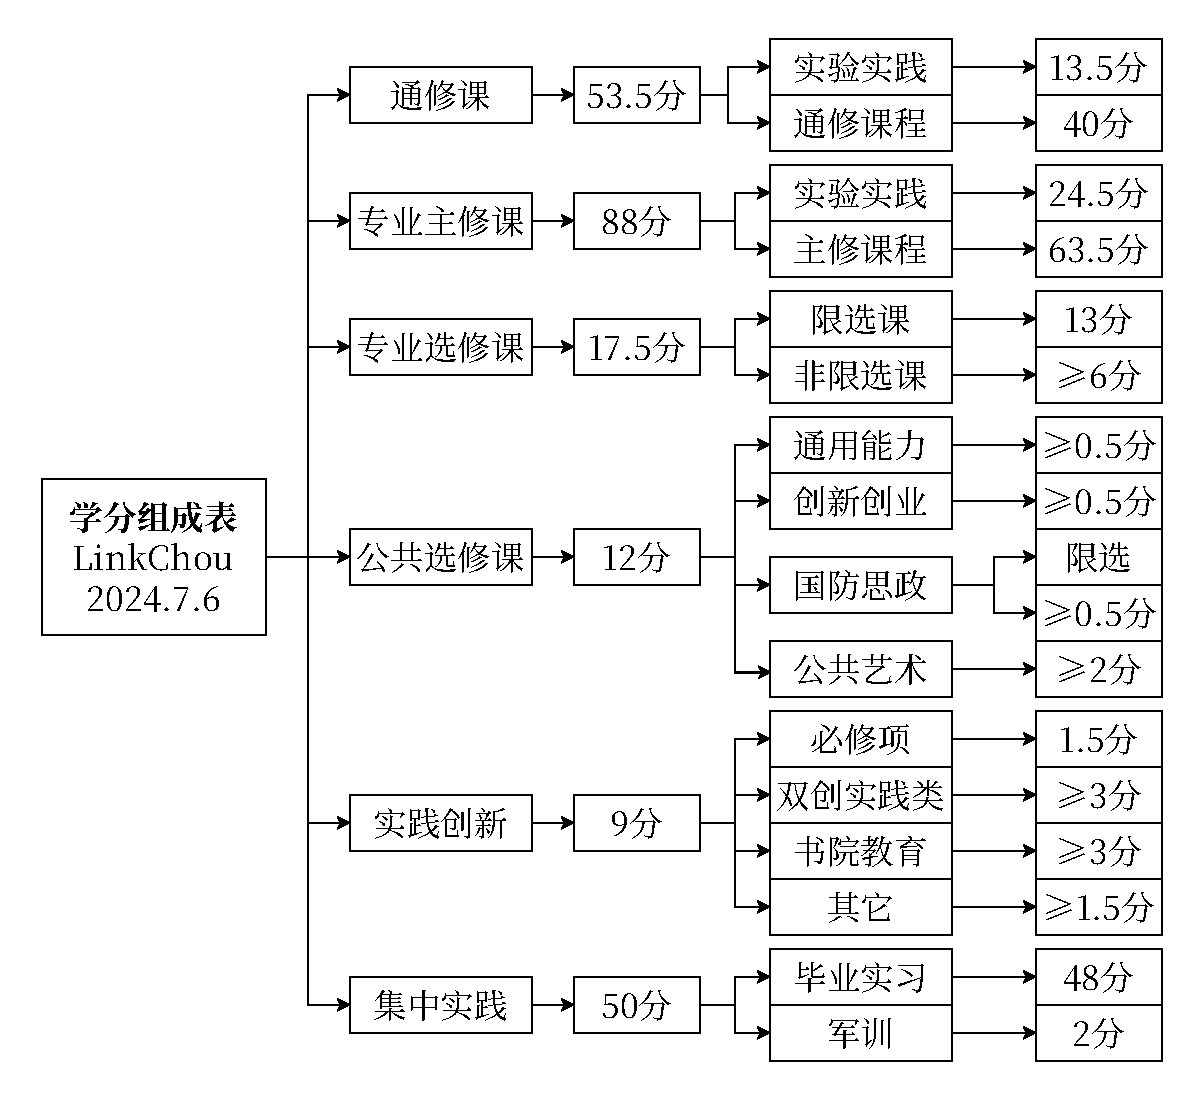
\includegraphics[width=\textwidth]{学分.pdf}%
    \label{credit}%
}

\subsection[留学、国际交流]{留学、国际交流}
如需出国留学或进行国际交流时该校要求出示平均绩点等相关证明,请咨询教务处相关事宜。

\section[缓考、补考与重修]{缓考、补考与重修}
\label{retake}

\subsection[补考]{补考}
\begin{enumerate}
    \item 必修课、限定选修课不及格(50 ≤ 分数 < 60)可以申请补考1次,仅计算卷面成绩,若及格则按60分计入综合成绩(折算为1绩点)
    \item 非限选课、公共选修课不及格需改选或重选,不予补考
    \item 每门课程仅1次补考机会(缺考除外),不额外收费
\end{enumerate}

\subsection[重修]{重修}
\begin{enumerate}
    \item 缓考或补考不及格者需要重修对应科目
    \item 必修课、限定选修课不及格(分数 < 50)需重修对应科目
    \item 非限选课、公共选修课不及格可以选择重修或直接改选其他科目
    \item 最终分数以实际为准(计入新的平时分)
\end{enumerate}

\subsection[缓考]{缓考}
缓考科目的分数以考试为准(计入平时分),缓考申请教程参见《山东第二医科大学指南》,此处不再赘述。

\section[关于学位证、毕业]{关于学位证、毕业}
\begin{enumerate}
    \item \textbf{存在以下情况将无法获得学位证}
          \begin{enumerate}
              \item 修不够每项对应的学分
              \item 平均绩点 < 2分
              \item 受过记过及以上处分
              \item 其他不符合相关要求的情况
          \end{enumerate}
    \item 留级:累计两次获得三级学业预警的将会留级
    \item 无法毕业:三阶段考试最终分数不及格
\end{enumerate}

\part[其他事项]{其他事项}

\section[转专业]{转专业}

注:本小节依据教务处2024年5月21日发布的《山东第二医科大学2024年普通全日制本科学生转专业工作方案》简化。该规定每年不一,如有变动,以教务处政策为准。

\subsection[转专业条件]{转专业条件}
\begin{enumerate}
    \item 取得学籍的普通全日制一年级本科在校生
    \item 未受处分、思想过硬、符合体检要求
    \item 第一学年必修课和专业限定选修课平均成绩在本专业排名前30\%,且未挂科
    \item 以特殊招生形式录取的学生,国家有相关规定或者录取前与学校有明确约定的(如公费医学生等),不得申请转专业
\end{enumerate}

\subsection[考试科目]{考试科目}
思政、英语\footnotemark、数学,比例为1:1:1,考试时间150分钟,总分为150分
\footnotetext{高考小语种考生可选择小语种替代英语,需在报名时备注,不备注者参加英语考试。}

\subsection[流程]{流程}
\begin{enumerate}
    \item 核算学生第一学年学习成绩并公示各类数据
    \item 8月31日开始报名
    \item 9月5日组织考试(地点详见相关通知)
    \item 9月6日~10日公示录取名单\footnotemark
          \footnotetext{按照“分数优先,遵循志愿,一次投档”的原则进行录取,成绩排名在专业应考人员中居前20\%者取得转专业资格。}
    \item 9月11日~12日报到
\end{enumerate}

\section[关于选修课的补充说明]{关于选修课的补充说明}
\begin{enumerate}
    \item 选修课分专业选修和公共选修两大类(详见学分组成表\uref{credit}),\textbf{推荐在大一全年、大二上学期就把各类选修学分全都修满},这样就不用在后面学业愈重的情况下兼顾选修课的学习了,可以专心针对专业课程进行深入学习
    \item 专业选修课有限选和非限选之分,限选的课程无需操心,教务系统会自动选课,只需要保证非限选的课程学分达标即可
    \item 公共选修课每一类都要选至少一门,且需要满足总分,其中部分类别还有额外要求(详见学分组成表),国防教育类有国家限选课程(到时候看具体通知,会说的很明白的)
    \item 公共选修课有一部分是在教室上的,还有一部分是线上课程(使用“知到”app进行学习,大多数有平时分),可以根据自己的实际情况选择
\end{enumerate}

\section[班级综测]{班级综测}
\label{class_evaluation}
\begin{enumerate}
    \item 综测是综合素质测评的简称,一般包含学习、活动、比赛等大类,加权相加后为得分,各年级要求不一,详见学生手册
    \item 班级综测是用于考核各班表现的评判指标,与班级评优评先、班集体评优评先名额分配、见习点分配\footnotemark 强相关,每学期计算一次,截至见习
          \footnotetext{以截至见习之前的各学期平均班级综测成绩计算班级排名,公费班级根据本年级政策进行。}
    \item 班级综测直接决定本班级同学后期学习和生活所在的医院规模、等级和生活条件,请大家务必重视\\
          例如:宿舍有无空调、暖气、洗衣机,是否提供插座,是否有早操和晚查寝\footnotemark 等
          \footnotetext{这意味着能否在外租房居住。}
\end{enumerate}

\section[临床医学专业三阶段综合考试]{临床医学专业三阶段综合考试}
大一的基础课程是一切的根基。

因临床医学专业无毕业论文,为检测学生阶段知识掌握情况,学校实行了临床医学专业三阶段综合考试(下简称“三阶段考试”)的方法。此外,三阶段考试如果最终综合分数不及格,将无法毕业;若二阶段考试不及格,将无法进入医院实习;其他规定详见本节最后的\uref{other_rules_exam}小节。

\subsection[第一阶段综合考试(基础医学综合考试)]{第一阶段综合考试(基础医学综合考试)}
\begin{enumerate}
    \item 考察内容:组织胚胎学、病理学、病理生理学、解剖学、生理学、生物化学、药理学、医学免疫学、医学微生物学
    \item 考查时间与方式:第6学期进行,机考或笔试
    \item 其他信息:时长2.5小时,共300题,满分100分
\end{enumerate}

\begin{tblr}[
        long,
        caption = {一阶段考试详表},
    ]{
        cells = {c,m},
        rowhead = {1},
        row{1,Z} = {cmd=\bfseries},
        hline{1-2,Z} = {-}{1pt},
    }
    考试内容     & A1型题   & A2型题   & B1型题   & 总计     \\
    组织胚胎学   & 45~50\% & 35~40\% & 15~20\% & 5~10\%  \\
    病理学       & 45~50\% & 35~40\% & 15~20\% & 10~15\% \\
    病理生理学   & 45~50\% & 35~40\% & 15~20\% & 10~15\% \\
    解剖学       & 45~50\% & 35~40\% & 15~20\% & 10~15\% \\
    生理学       & 45~50\% & 35~40\% & 15~20\% & 10~15\% \\
    生物化学     & 45~50\% & 35~40\% & 15~20\% & 10~15\% \\
    药理学       & 45~50\% & 35~40\% & 15~20\% & 10~15\% \\  %避免自动换行不对劲导致出现vbox warning
    医学免疫学   & 45~50\% & 35~40\% & 15~20\% & 10~15\% \\
    医学微生物学 & 45~50\% & 35~40\% & 15~20\% & 10~15\% \\
    总计         & 45~50\% & 35~40\% & 15~20\% & 100\%
\end{tblr}

\subsection[第二阶段综合考试(临床医学综合考试)]{第二阶段综合考试(临床医学综合考试)}
\begin{enumerate}
    \item 考察内容:
          \begin{enumerate}
              \item 理论考试:
                    \begin{enumerate}
                        \item 基础医学:病理学、解剖学、生理学、生物化学、药理学、医学免疫学、医学微生物学
                        \item 临床医学:内科学、外科学、妇产科学、儿科学
                        \item 医学人文:医学伦理学、医学心理学
                        \item 预防医学:预防医学
                    \end{enumerate}
              \item 技能考试:病史采集、体格检查、基本操作技能、沟通交流能力、人文关怀
          \end{enumerate}
    \item 详情考试形式、考试时间、试题数量以“国家医学考试中心”通知为准
    \item 下附往年二阶段理论考试详表
\end{enumerate}

\begin{tblr}[
        long,
        caption = {二阶段理论考试详表},
    ]{
        cells = {c,m},
        rowhead = {1},
        row{1,Z} = {cmd=\bfseries},
        hline{1-2,Z} = {-}{1pt},
    }
    考试内容 & A1型题   & A2型题   & B1型题   & 总计     \\
    基础医学 & 45~50\% & 35~40\% & 15~20\% & 40~45\% \\
    临床医学 & 20~25\% & 70~75\% & 3~5\%   & 40~45\% \\
    医学人文 & 45~50\% & 35~40\% & 15~20\% & 5~10\%  \\
    预防医学 & 35~40\% & 55~60\% & 3~5\%   & 5~10\%  \\
    总计     & 30~35\% & 50~55\% & 10~15\% & 100\%
\end{tblr}

\begin{tblr}[
        long,
        caption = {二阶段实践考试详表},
        note{1} = {沟通能力、人文关怀等医学人文素养的考核融合到各站,分值约占15\%。},
    ]{
        cells = {c,m},
        rowhead = {1},
        row{1,Z} = {cmd=\bfseries},
        hline{1-2,Z} = {-}{1pt},
    }
    考站 & 考试内容\TblrNote{1} & 考试方式 & 考试时间 & 分值 \\
    1站  & 病史采集             & SP       & 10分钟   & 20   \\
    2站  & 病史采集             & SP       & 10分钟   & 20   \\
    3站  & 体格检查             & 操作     & 10分钟   & 15   \\
    4站  & 体格检查             & 操作     & 10分钟   & 15   \\
    5站  & 基本操作             & 操作     & 10分钟   & 15   \\
    6站  & 基本操作             & 操作     & 10分钟   & 15   \\
    合计 &                      &          & 60分钟   & 100  \\
\end{tblr}

\subsection[第三阶段综合考试(毕业综合考试)]{第三阶段综合考试(毕业综合考试)}
\begin{enumerate}
    \item 考察内容:
          \begin{enumerate}
              \item 理论考试:内科学、外科学、妇产科学、儿科学
              \item 技能考试:职业素质、病史采集、体格检查、基本操作、辅助检查、病例分析
          \end{enumerate}
    \item 考查时间与方式:实习结束、毕业前进行,笔试或机考、面试
    \item 其他信息:理论考试时长2小时,共200题,满分100分;技能考试时长1小时,形式为客观结构化临床考试(OSCE),共12~16站,满分100分
\end{enumerate}

\begin{tblr}[
        long,
        caption = {三阶段理论考试详表},
    ]{
        cells = {c,m},
        rowhead = {1},
        row{1,Z} = {cmd=\bfseries},
        hline{1-2,Z} = {-}{1pt},
    }
    考试内容 & A1型题   & A2型题   & A3型题   & 总计     \\
    内科学   & 45~50\% & 25~30\% & 25~30\% & 35~40\% \\
    外科学   & 45~50\% & 25~30\% & 25~30\% & 35~40\% \\
    妇产科学 & 45~50\% & 25~30\% & 25~30\% & 10~15\% \\
    儿科学   & 45~50\% & 25~30\% & 25~30\% & 10~15\% \\
    总计     & 30~35\% & 50~55\% & 10~15\% & 100\%
\end{tblr}

\subsection[相关规定]{相关规定}
\label{other_rules_exam}
\begin{enumerate}
    \item 补考:一阶段由基础医学院组织补考;二阶段由教务处组织考试;三阶段由临床医学院组织补考
    \item 成绩折合与毕业:各阶段理论考试成绩按照2:4:4的比例折算后,作为毕业考试理论成绩;二、三阶段技能考试成绩按5:5折算后作为毕业考试技能成绩;不及格者不予毕业
    \item 综测与奖学金:一、二阶段成绩纳入个人综测和奖学金评定
    \item 实习:二阶段合格者可以进入医院实习,否则需要通过实践教学管理处和临床医学院组织的实习准入考试
\end{enumerate}

\section[杂项]{杂项}
\begin{enumerate}
    \item \textbf{大一不允许参加四级考试,大二才能报名四六级}
    \item 关于奖学金:本校有国家奖学金、校长奖学金、校级3等级奖学金等\\
          请注意,目前学校仅能通过本人身份开通的、已开户的、账户已激活的、无异常的工商银行储蓄卡发放奖学金,详情政策可咨询学校财务处。
\end{enumerate}